\chapter{Community concept}
\label{CommunityConcept}
%I dette kapitel skal konceptet bag TonePrint communitiet forklares med udgangspunkt i at der tilsidst skal tages et valg af hvilken det vi skal hjælpe med at udvikle.\\
Based on the description of TC Electronics development process in \autoref{InterviewConclusion}, the current task is to develop conceptual models, which describes the functionalities and use cases of the TonePrint Community. The scope of this phase is to discover which tasks that lay ahead the development of the TonePrint Community, while focusing on user involvement and user experience. \\

\section{Conceptual model}
\label{ConceptualModel}
In \parencite[][17]{PDF:Henderson2012} a conceptual model is descried  as "\textit{A high-level description of an application. It enumerates all concepts in the application that users can encounter, describes how those concepts relate to each other, and explains how those concepts fit into tasks that users perform with the application}".\\
In order to create the conceptual model of the TonePrint Community, some decisions have to be taken about functions, features and interactions, which hasn't been made on a business level yet. These decisions are therefore not fixed, in term of the final product, but will serve its purpose for this project. The decisions are based on the interviews in \autoref{ThemanticAnalysis} and reflects ideas and opinions from the development team.

\subsection{The TonePrint Concept model}
\label{TonePrintConceptualModel}
When creating the conceptual model we need to look at the task domains in which the user till perform activities to reach their goal. Different users have different purposes for using the community and therefore will there be more than one task domain to consider, while designing the community. \\
At first we look at the different groups of users for the TonePrint concept, as described in (\footnote{Appendix or analysis of interview}). On \autoref{fig:TonePrintUserConpt} it's depicted how users of the TonePrint concept are categorized into three groups, Pedal only users, TonePrint Users and TonePrint creators. The 'Pedal only users' are the users whom own a TonePrint pedal, but doesn't use the TonePrint functionalities of the pedal and just are using it as a regular pedal. We define the TonePrint Users as those who use the TonePrint concept to find and beam Artist TonePrints to their pedals. These users are therefore connected to the Artist Library of the TonePrint application. We define the TonePrint Creators as those whom uses the TonePrint concept to create User TonePrints, which they can use with their pedals. These users are therefore connected to the Editor and the User TonePrint Library. The connecting arrow between TonePrint Users and Creators on \autoref{fig:TonePrintUserConpt} indicates that these users isn't necessary different people, but might be the same user using the system differently. 

\begin{figure}[H]
	\centering
	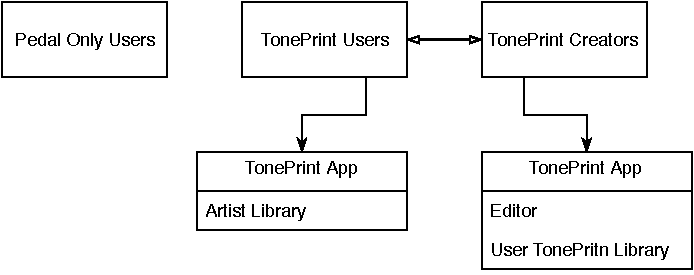
\includegraphics[width=0.85\textwidth]{TonePrintConcept.pdf}
	\caption{This illustrates the different groups of users of the TonePrint concept}
	\label{fig:TonePrintUserConpt}
\end{figure}

The definition of the different user groups of the TonePrint concept will also be applied to the concept of the TonePrint Community, however are the 'Pedal Only Users' neglected in future models. This is because they aren't using the TonePrint functions and thereby don't have any use of the TonePrint Community. The features listed in \autoref{tab:ListOfCommunityFeatures} are suggested to accommodate both the TonePrint users and creators in the community. The features are based on the ideas and suggestions from the interview with development team in \autoref{ThemanticAnalysis}.

\begin{table}[H]
	\centering
\begin{tabular}[width=\textwidth]{c|l}
\textbf{Ref. nr} & \textbf{Features} \\ \hline
1 & Uploading TonePrints \\ \hline
2 & Categorize by tags \\ \hline
3 & TonePrint description \\ \hline
4 & Search \\ \hline
5 & Rate TonePrint \\ \hline
6 & Subscribe to user (Artist) \\ \hline
7 & User profile \\ \hline
\end{tabular}
\caption{The left column contains the number which is used to refer to the feature in the right column}
\label{tab:ListOfCommunityFeatures}
\end{table}

The features 1, 2 and 3 in \autoref{tab:ListOfCommunityFeatures} are all closely related and accommodates especially the task domain of the TonePrint Creators. The feature of uploading features are simply to enable user to upload TonePrints to the community, that they have created with the editor. This feature covers the main function requested by the users which is the ability to share TonePrint with each other. Feature 2, Categorizing by tags refers to the idea of letting users use tags to categorize the TonePrint they have uploaded. The purpose of these tags are to easily allow other users to identify which categories the TonePrint belongs to, which also enable users to find the discover tonePrints by searching on different tags/categories. Feature 3, TonePrint description allows the creator of a TonePrint to write about the TonePrint, similar to the descriptions of the Artist TonePrints in the current TonePrint application. The description might contain information about the parameter settings, inspiration, self-promoting text or likewise.

\begin{figure}[H]
	\centering
	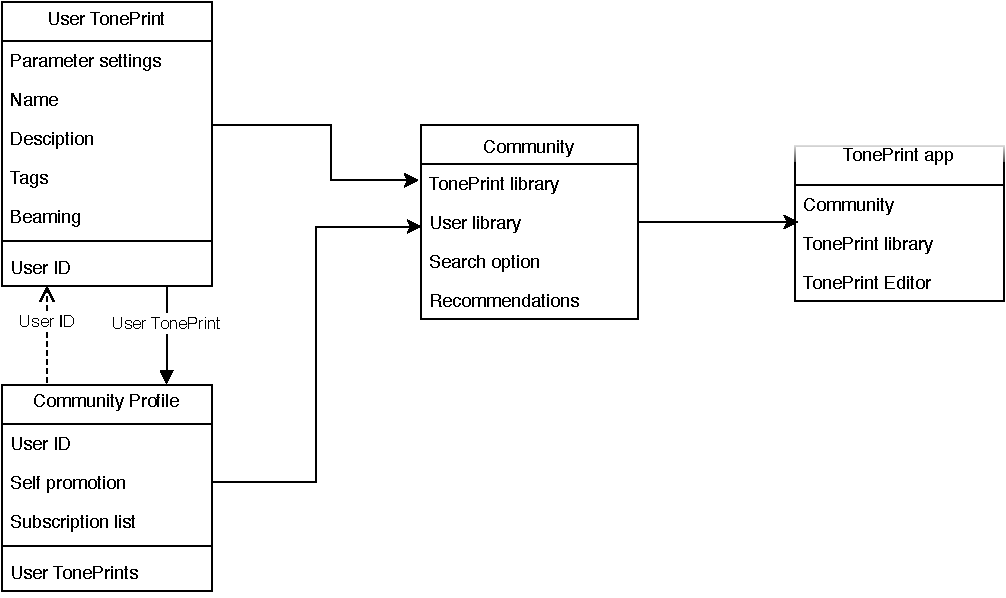
\includegraphics[width=0.85\textwidth]{CommunityFirstDraft.pdf}
	\caption{a graphical overview of the TonePrint Community concept}
	\label{fig:CommunityConceptualModel}
\end{figure}

\subsection{Use case}

\begin{figure}
	\centering
	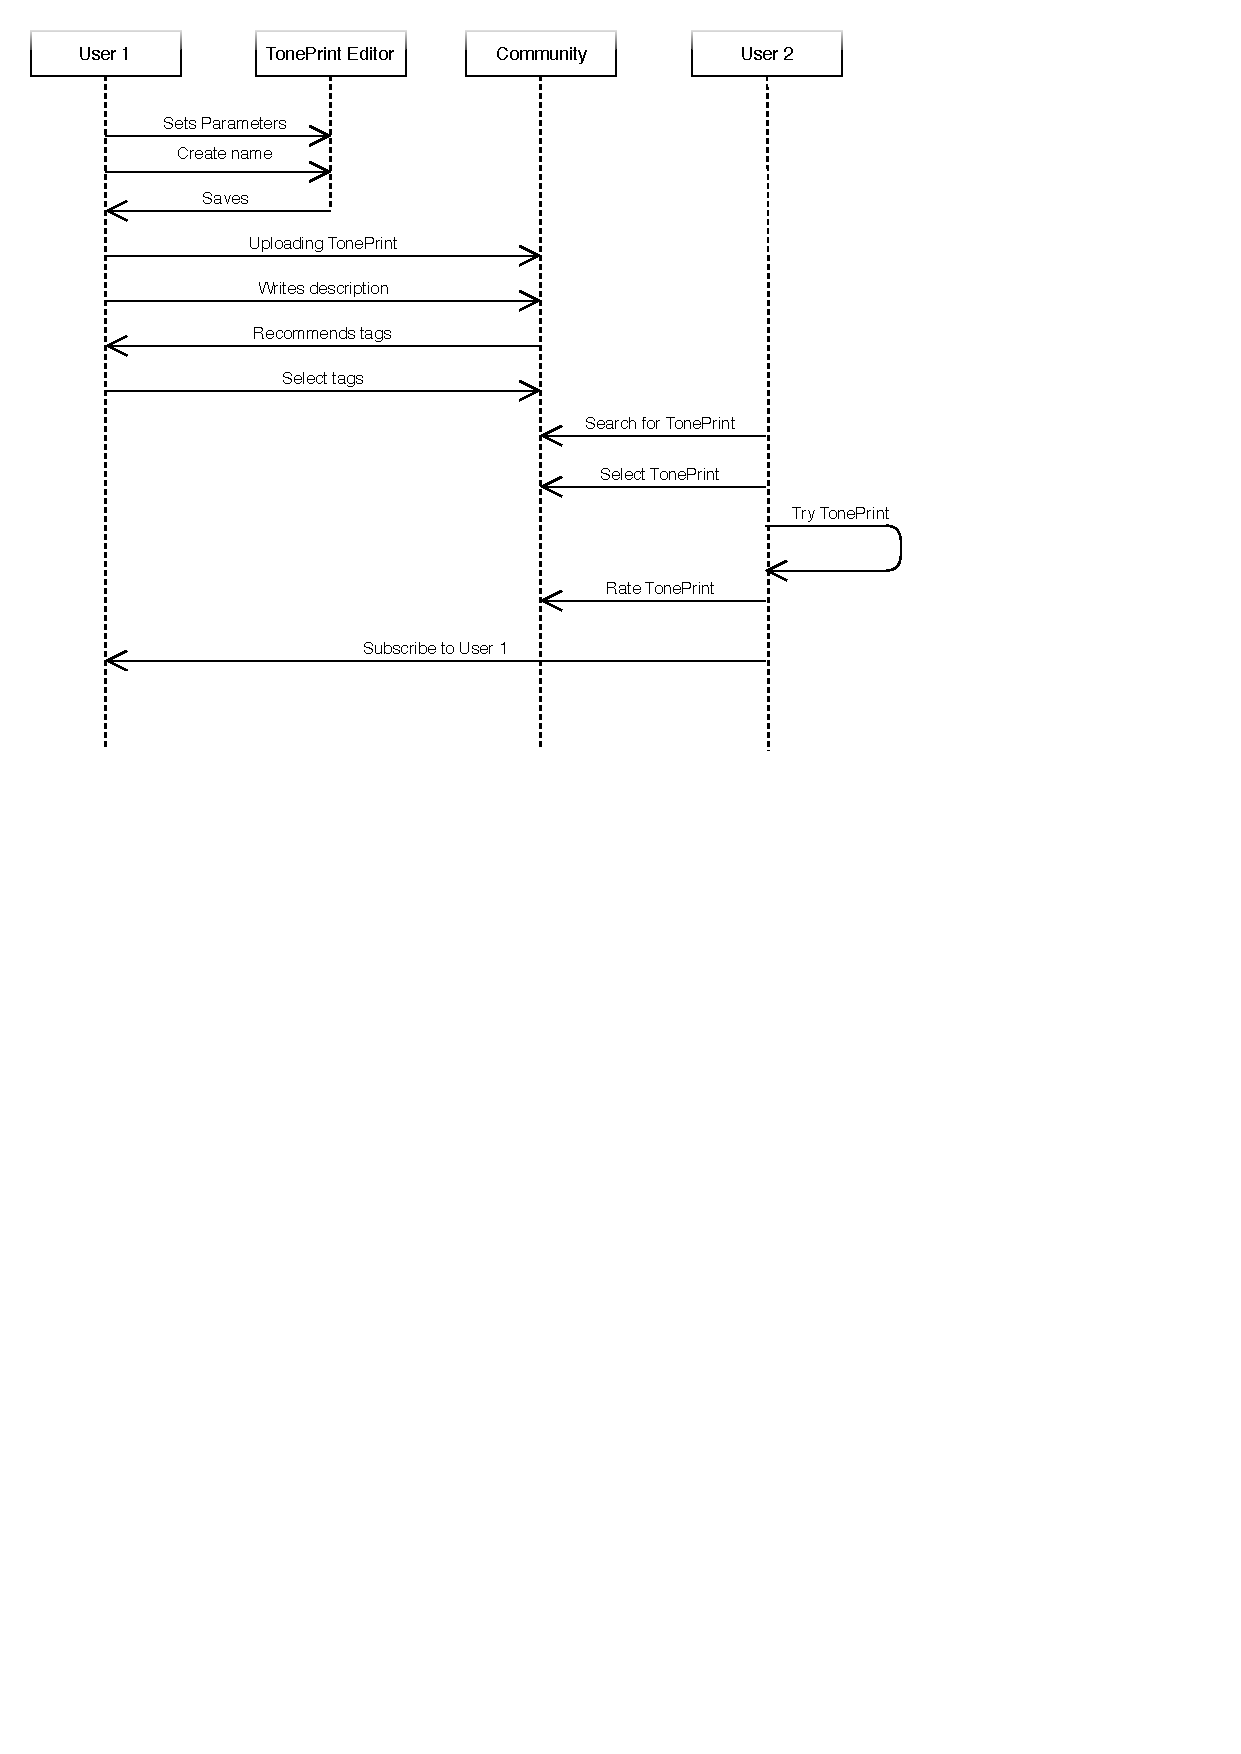
\includegraphics[width=0.85\textwidth]{CommunityUseCaseOne.pdf}
	\caption{a graphical overview of the TonePrint Community use case}
	\label{fig:CommunityConceptualUseCase}
\end{figure}